Unfortunately on this one, the plots out of R on such small scales caused some problems for both the titles and the labels.

Showing $k_max$ for $N = 10^1$ (left) and for $N = 10^2$ (right).

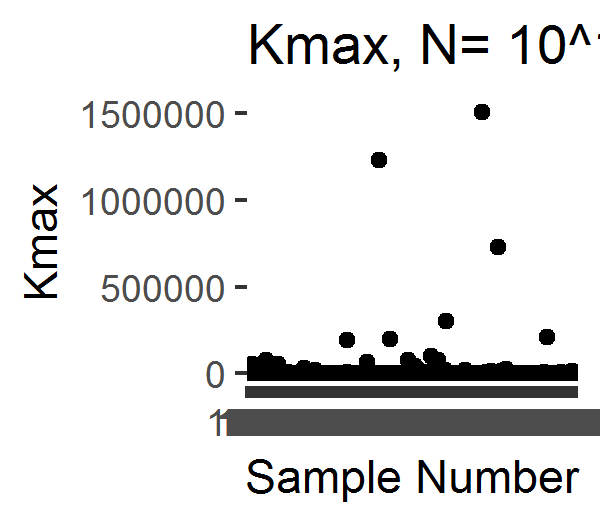
\includegraphics{../images/Problem6_10^1.png}
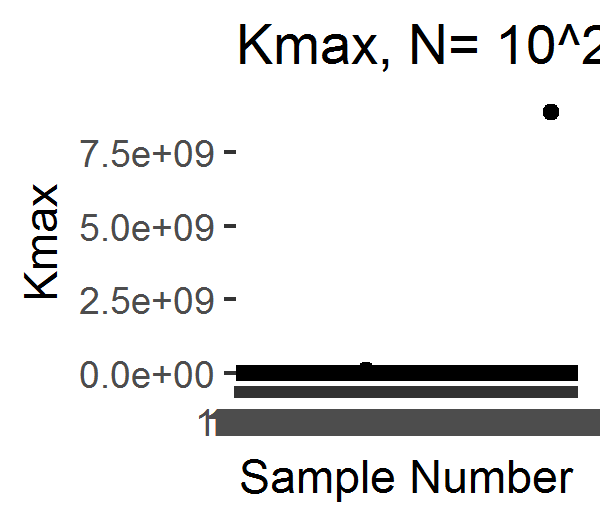
\includegraphics{../images/Problem6_10^2.png}

Showing $k_max$ for $N = 10^3$ (left) and for $N = 10^4$ (right).

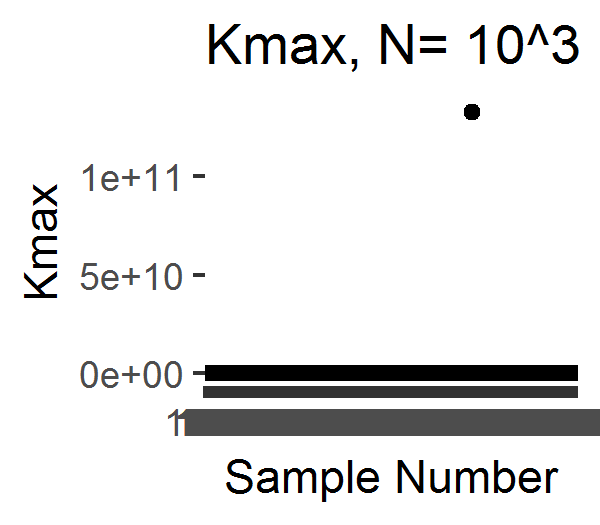
\includegraphics{../images/Problem6_10^3.png}
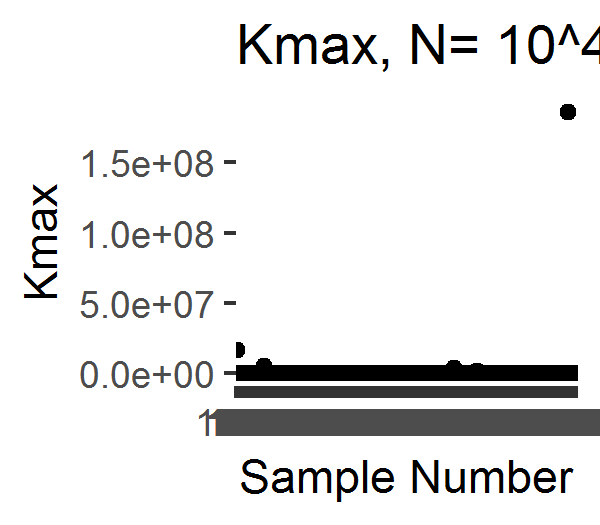
\includegraphics{../images/Problem6_10^4.png}

Showing $k_max$ for $N = 10^5$ (left) and for $N = 10^6$ (right).

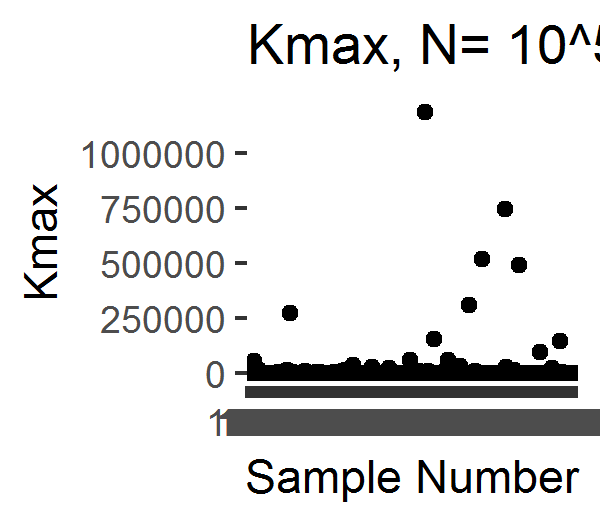
\includegraphics{../images/Problem6_10^5.png}
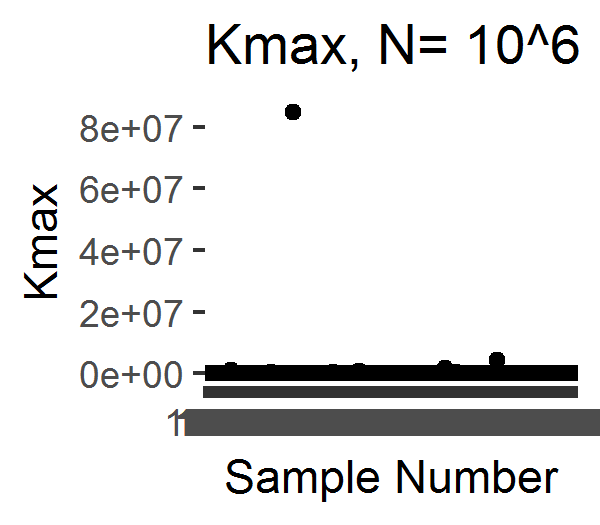
\includegraphics{../images/Problem6_10^6.png}

Unfortunately for this homework it seems that again, something is off. Here, unfortunately because of the nature of power law distributions I can't tell if it is the nature of the distribution but I assume it is probably a result of my algorithm. Here, I would expect from the averaging from 1000 simulation that any of the erratic behavior from the output of the power law distributions would be mitigated. Here, unfortunately, from my graph of the average for $k_max$, I don't see any relationship in the average value of $k_max$ in terms of the sample size.

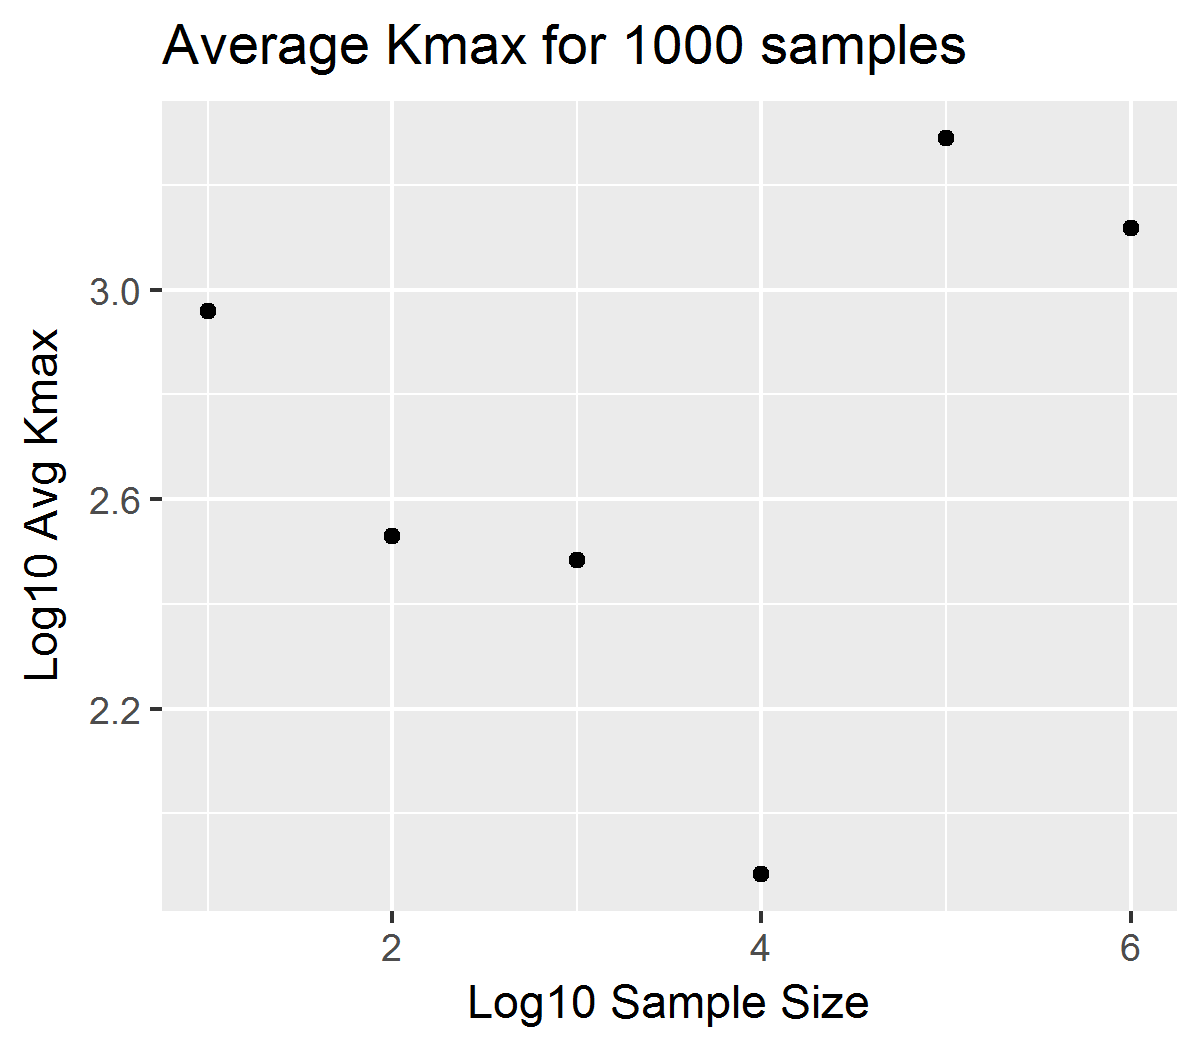
\includegraphics{../images/Problem6_average_max.png}